\chapter{Hypergraph Linguistic Model}
\label{chap:ling_net}
\begin{abstractchap}
In the previous chapter we presented the theoretical notions used in representing text through a distributional approach, the parameters, the models to implement them in real applications and the problems that naturally arise from these implementations. In this chapter we present and define the whole of our contributions. We organize this  chapter  in four parts: first, we introduce a state of the art on how the information contained in linguistic graphs is used for WSD/WSI and NER. Secondly, we introduce our model, addressing the limitations of classical language networks. Thirdly, we present a second state of the art on the combination  of contextual features in NLP with fusion techniques. Finally, we apply the proposed model to a corpus extracted from the English Wikipedia. We describe the process and the characteristics of the extracted network.
\end{abstractchap}
\minitoc

\begin{figure}
\centering
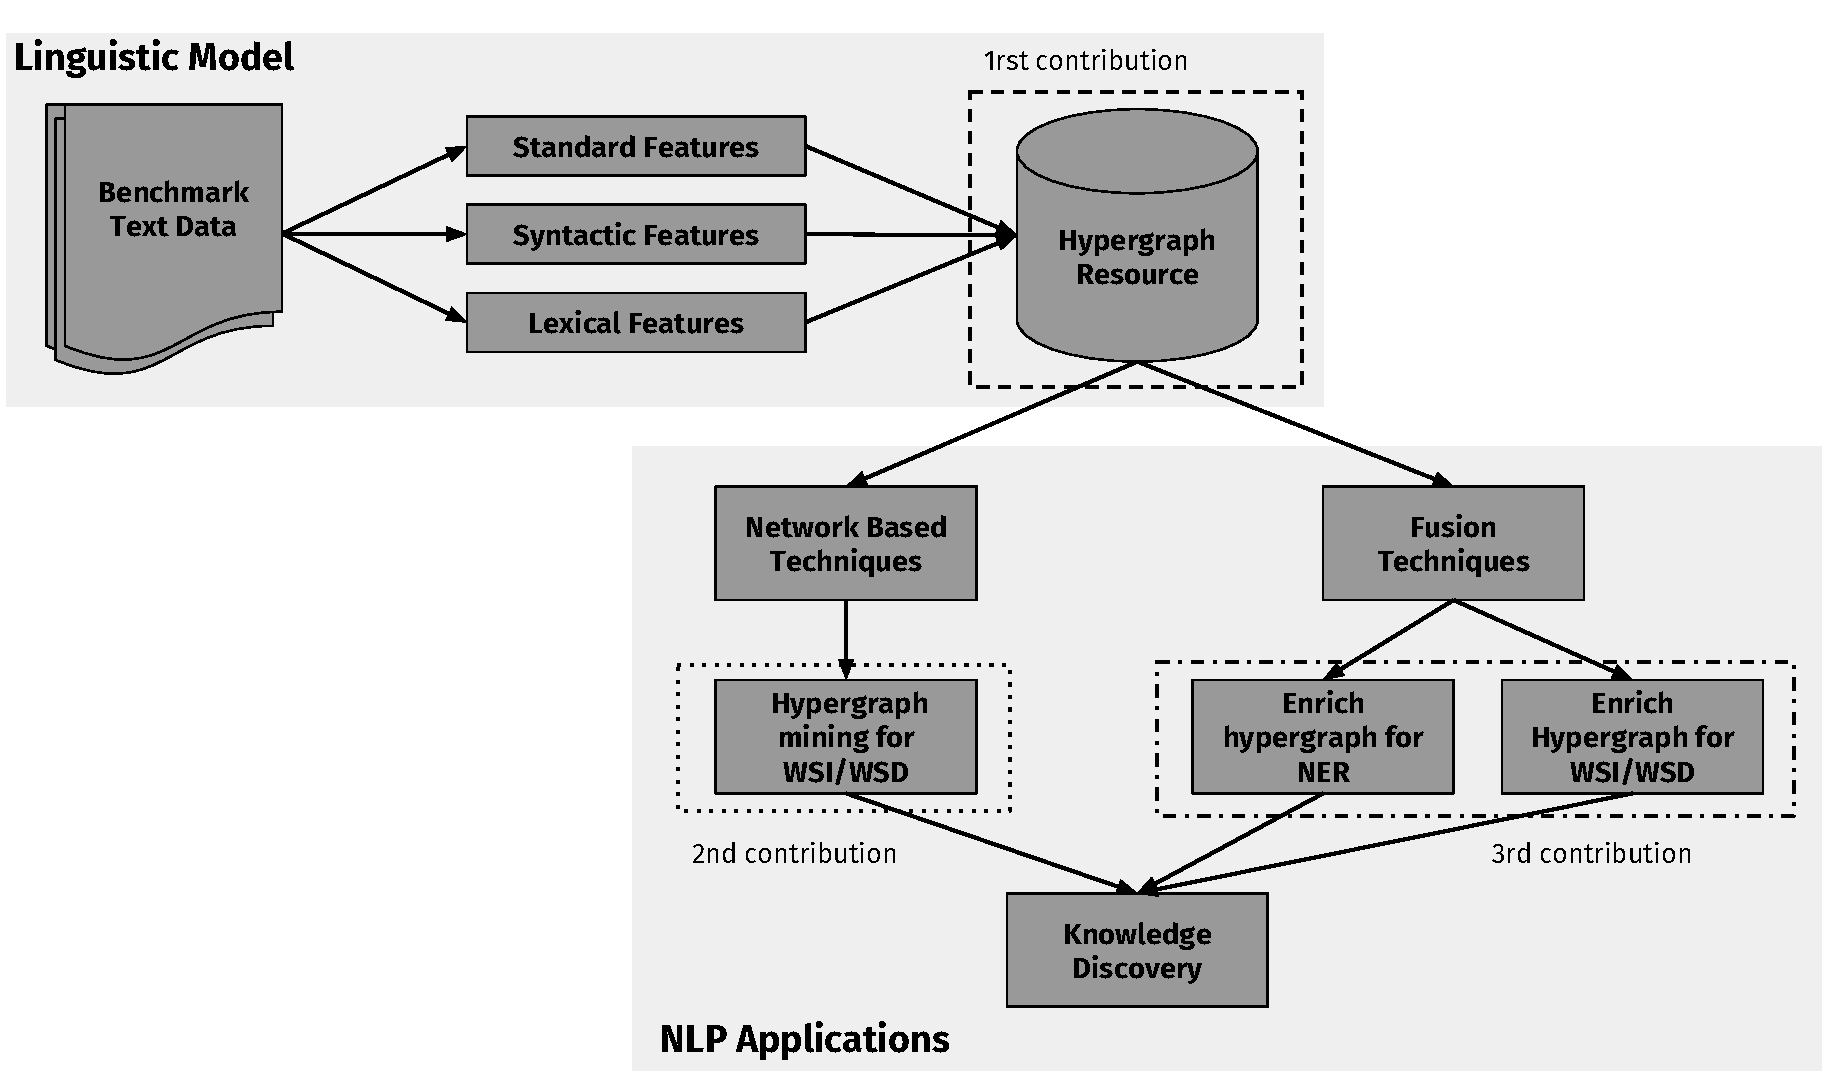
\includegraphics[width=1\linewidth]{./images/Chapitre3/main_diag.pdf}
\caption{Modular description of this dissertation}
\label{fig:maindiag}
\end{figure}
\section{Introduction}
A hypergraph linguistic model is the first core contribution of this thesis. We will describe the motivations and its characteristics below. On Figure \ref{fig:maindiag}, we can appreciate the block diagram of the ensemble of our propositions. At the top, we see that the hypergraph resource that we propose on this chapter is the stepping stone framework upon which we base the rest of our work. The model entails three  important characteristics: (1) the possibility to leverage three types of information. That is, syntactic, lexical  and what we will call standard features (explained later on), (2) as the words will be linked together, there is an inner structure that will emerge from the model, finally (3) the relations will between words are sparse. The tree of them are addressed with our propositions, while testing their practicality with well-established task domain corpora, which we use as benchmark input data in our experiments. These approaches, 2nd and 3rd contributions, are described in the next chapter.

In order to contextualize our proposition, we begin with the state of the art on how linguistic networks are employed in the literature. We are interested on those networks previously covered: lexical, syntactical and semantic co-occurrence networks. We give emphasis to two aspects: how the inner structure is used to solve the tasks at hand, and what type of graph-based algorithm is used. The literature on graph-based approaches for NLP is vast, we thus focus specifically on semantic tasks, notably Word Sense Induction and Disambiguation, and Named Entity Recognition. We chose these two tasks as we focus on both of them for the rest of our contributions. Next, we introduce our model, how to build it  and its properties. 

\section{Linguistic Networks in Semantic NLP Tasks}



We present here an overview of linguistic network's related work. We discuss what and how different methods are used with language networks to extract knowledge from their structural properties. Finally, we discuss the limitations of the current propositions and the advantages of the model we propose.
%\minitoc



\paragraph{Using Lexical Co-occurrence Networks}

Lexical Co-occurrence Networks (LCN) are  popular  since they do not require any special treatment to obtain them, just the input corpus. It is then natural that truly-unsupervised\footnote{Without the need of human-crafted semantic networks.} word sense induction approaches leverage these type of networks, and in return, the distributional hypothesis, to automatically discover senses for a given target word. That is why several WSI methods \cite{2004.Veronis,2007.Klapaftis.UOY,2010.Navigli.InducingWordSenses.Triangles,2008.Klapaftis.WSIUsingCollocations,2011.DiMarco.Navigli.ClusteringWebSearch,2011.Jurgens.WSICommunityDetection} are tightly related to LCNs. 
The cited works use a LCN as described before while other works such as \cite{2007.Navigli.GraphConnectivity,2014.Tao.Qian.LexicalChainHypergraphWSI} represent, as we do,u the co-occurrence by means of a hypergraph scheme. In short, a hypergraph structure is a graph generalization where an edge (called hyperedge) can link more than two vertices per edge and thus it is able to provide a more complete description of the interaction between several nodes \cite{estrada2005}.

In their paper, given an input document with several contexts for each target word, they first group together the contexts via a topic-modeling technique. Thus, each context is assigned a particular group (in this case, a topic). Secondly, a hypergraph is built where the vertices represent contexts and the hyperedges link two nodes together if they share the same topic. Thirdly, the hypergraph is clustered and the words of each context (of each node) are used to build vectorial representations

WSI systems generally perform four steps. Given an input text with a set of target words and their contexts (target words must have several instances throughout the document to cluster them), the steps are the following:

\begin{enumerate}
\item Build a LCN, assigning tokens as nodes and  establishing edges between them if they co-occur in a given context (usually if they both appear in the same sentence),
\item Determine the weights for each edge according to a frequency metric,
\item Apply a graph clustering algorithm. Each cluster found will represent a sense of the polysemous word, and
\item Match  target word instances with the clusters found by leveraging each target word context. Specifically, assign a cluster (a sense) to each instance by looking at the tokens in the context.
\end{enumerate}

As with semantic networks, not only WSD or WSI can be solved with LCNs. Finding semantic associated terms in a corpus is a critical step in several NLP systems. This task is solved in the system proposed by \cite{2011.Haishan.AHypergraphbased}. They also use a LCN although instead of a co-occurrence graph, they also employ a co-occurrence hypergraph, where nodes represent words and edges describe co-occurrence at the paragraph level.  In this work, they use such structure to find related terms in a given corpus. In order to do it, they mine the hypergraph as in a frequent itemsets problem, where the items are the words from a text. The method consists in first finding similar itemsets by means of measuring similarity between nodes. Once the 2-itemsets are found, they induce a graph from the original hypergraph by drawing edges between nodes that have a similarity superior to an arbitrary threshold. Lastly, in order to find $k$-itemsets ($k > 2$), the find either complete or connected components in the induced graph. 



As with WSD, while the LCNs used are mostly the same among approaches, there are certain moving parts that make up the difference between WSI approaches. The most common differences that can arise are:

\begin{itemize}
\item The clustering algorithm to find senses in the LCN graph.
\item The technique used to match context words to clusters.
\item The weight used in the graph edges.
\end{itemize}



\paragraph{Using Syntactic Co-occurrence Networks}

A network representation that is on the border line between being a LCN and a SCN is that of \cite{2013.Bronselaer.TextAnalysisWithGraphs}. They  propose a graph document modelization. In their network, nodes represent words and edges their co-occurrence, as any LCN. Still, their graph resembles a SCN because the edges may represent one of three types of words: either prepositions, conjunctions or verbs. As a result,  they need to first extract syntactic information from a document, namely the part-of-speech tags of each word. They find the most relevant words of a given text by ranking the nodes of the graph. The words that best represent a document can be used to summarize it, as they show in their work.

Approaches based on SCN are rarely used in WSD or WSI systems, and therefore they are an interesting research avenue to explore.




\paragraph{Using Semantic Networks}

Word sense induction is indeed a task usually solved using semantic networks, specially Wordnet (and to a lesser extent, BabelNet) \cite{2004.Mihalcea.SemanticNetworkPageRank,2007.Sinha.Mihalcea.Unsupervised,2007.Tsatsaronis.WSDwithSpreading,2007.Navigli.GraphConnectivity,2008.Agirre.Multilingual,2008.Klapaftis.WSIUsingCollocations,2009.Agirre.PersonalizedPageRankWSD,2010.Klapaftis.WSD.WSD.HierarchicalGraphs,2010.Siberer.GraphCooccurrenceWSD,2014.Moro.Navigli.EntityLinking_WSD}. Given an input text with a set of ambiguous target words to process, these approaches follow a two-step algorithm:
\begin{enumerate}
\item Link target words (usually nouns, skipping stop-words and functional words) with their corresponding  sense (or synset in the case of WordNet-like dictionaries) and extract their vertices and edges into a new, smaller, SN. 
\item Apply a node ranking technique, usually a random-walk-based method, and select, for each ambiguous word in the input text,  its top ranking synset node as the correct sense.
\end{enumerate}

The amount of edges a SN has grows depending of the size of the version of Wordnet used or the level of polysemy of a given word. In order to avoid redundancy or contradiction between  linking nodes, \cite{2004.Mihalcea.SemanticNetworkPageRank,2007.Navigli.GraphConnectivity} applied pruning techniques to avoid \textit{contamination} while calculating ranking metrics in order to define a pertinent sense. Regarding edge similarity measures,  in  \cite{2007.Sinha.Mihalcea.Unsupervised, 2007.Tsatsaronis.WSDwithSpreading} they test some metrics individually and also combined. They found that the best results are indeed obtained when several metrics are used at the same time.

%Other semantic tasks can also be solved using a SN. For example, Entity linking \cite{2014.Moro.Navigli.EntityLinking_WSD}. In their work, they leverage the BabelNet LKB to jointly disambiguate and link polysemous words to Wikipedia articles. 

Concerning the measure of semantic affinity between two terms, in \cite{2009.Yeh.Wikiwalk} they quantify word similarity by means of projecting them into a Wikipedia space. First, they represent each word by a vector representing its most pertinent pages,  and then they calculate a vectorial similarity measure between them.

%In \cite{2013.Matuschek.Gurevych.Dijsktra.WSA} they propose a technique that aligns SNs, i.e., they link senses from two different networks. This task is called word sense alignment. Several SNs are used (Wordnet, Wikipedia, Wiktionary, etc.) thus nodes can represent synsets, articles, or concepts. The links may depict semantic relations or may be links joining two concepts or pages together. Their approach aims to find the shortest path between nodes of any two given SNs while leveraging already existing links between  equal concepts found in both SNs.



Finally, extracting entities from text can also benefit from the use of SNs. The work proposed by  \cite{2013.Kivimaki.AGraph-BasedApproach} aims to extract technical skills from a document. Again, using Wikipedia as SN, they first represent each article and the input document in a token vector space model.  Next, they find the document top 200 similar pages by calculating the cosine similarity between the document and each page. This serves to extract a Wikipedia subgraph which is used to calculate the most relevant pages for the entry document. Finally, the top pages are filtered by means of selecting those articles that actually represent a skill using a fixed list of skill-related tokens. Once again, the nodes represent Wikipedia articles and the edges the hyperlinks that join them.


The cited methods vary in how they make use of their SN, not so much in the network per se. These differences boil down to three aspects:
\begin{bulletList}
\item Type of relationship implied by the edges linking the nodes of the network, 
\item The algorithm used to rank the nodes after the semantic network is built, and
\item The weight assigned to each edge.
\end{bulletList}

\paragraph{Using Heterogeneous Networks}

Even though this kind of structure seems to open new avenues of research in the semantic analysis domain, only few explicitly take advantage of them, as is the case of \cite{2013.Saluja.Graph-BasedUnsupervisedLearning}. In their approach, they build a graph that links together features with words, and discover similarity measures that leverage the multi-typed nature of their network.


\subsection{Algorithms used in Linguistic Networks}

We have discussed until now the different types of networks from a content point of view. In this subsection, we address the details of the graph-based algorithms used to solve semantic NLP tasks. In this section we will cover the details of four different types of graph algorithms.

%\paragraph{Notation}
%In this section we will be referring to a connected undirected graph, which we denote by $G = (V,E,W)$. The graph $G$ has vertex set $V$, edge set $E$ where $|V|=n$, $|E|=m$, and the matrix $W\in\mathbb{R}^{n\times n}$, with $w_{u,v} \geq 0$, defines any kind of weights in the graph.


\paragraph{Edge Weights}

We begin by describing the metrics used to determine similarity between nodes, usually stored as edge weights. As stated in the previous sections, most of the metrics are frequency based, specially when dealing with LCNs. The main idea of these measures is to assign a weight that decreases as the association frequency of the words increases. Among these measures, the most popular are the Dice  coefficient \cite{2010.Navigli.InducingWordSenses.Triangles,2011.DiMarco.Navigli.ClusteringWebSearch,2013.DiMarco.Navigli.ClusteringGraph-BasedWSI}, normalized pointwise mutual information \cite{2013.Hope.GradedWSI}, and a graph-adapted tf-idf variant \cite{2007.Tsatsaronis.WSDwithSpreading} which aims to give importance to frequent edges while also favoring those that are rare.

Edge weights can also be calculated when the vertices of a network do not represent words. Such is the case of \cite{2010.Klapaftis.WSD.WSD.HierarchicalGraphs}, where nodes represents a target word context (set of tokens around an ambiguous word). This time the Jaccard index is used to quantify similarity between them while considering how many words are shared between a pair of context nodes.

When the nodes represent synsets (or concepts), certain approaches leverage only the intrinsic nature of the network connections, leveraged by random walk algorithms, without explicitly using  weighted edges \cite{2004.Mihalcea.SemanticNetworkPageRank}. 
 On the other hand, there are techniques that assign a frequency-based weight to represent the importance of a semantic relation, particularly those found in the reviews  by \cite{2007.Sinha.Mihalcea.Unsupervised,2007.Navigli.GraphConnectivity}, where several weights are tested.

A  more sophisticated approach to edge weighting is proposed in \cite{2013.Saluja.Graph-BasedUnsupervisedLearning} where they employ  custom-defined functions in order to learn the most appropriate edges' weights for a given set of seed vertices inside a network. The main idea  is to enforce \textit{smoothness} (keeping two nodes close if they have related edges) across the network.

As a way to rank edges according to their importance, the ratio of triangles (cycles of length 3), squares (cycles of length 4), and diamonds (graphs with 4 vertices and 5 edges, forming a square with a diagonal) in which an edge participates are calculated \cite{2010.Navigli.InducingWordSenses.Triangles,2013.DiMarco.Navigli.ClusteringGraph-BasedWSI}. Once the top edges are found, they create a subgraph containing only these edges (and its corresponding vertices).

Finally, instead of applying weights to edges, a case where  nodes are weighted can be found in \cite{2013.Kivimaki.AGraph-BasedApproach}. They measure and remove popular nodes in order to avoid their bias during the application of their random walk approach.




 

\paragraph{Graph Search}
Usually, in a WSD approach, the first step to follow is to build a graph from a LKB. The goal is to explore the semantic network and find all the senses linked to  those found in the context of an ambiguous word. Aside from custom search heuristics applied by certain works \cite{2006.Agirre.TwoGraph-basedAlgorithms,2007.Sinha.Mihalcea.Unsupervised,2009.Agirre.PersonalizedPageRankWSD}, researchers also use well-known graph techniques such as depth-first search \cite{2007.Navigli.GraphConnectivity}, breadth-first search \cite{2008.Agirre.Multilingual} and even the Dijsktra  algorithm to find the group of closest senses in the network \cite{2013.Matuschek.Gurevych.Dijsktra.WSA}.


\paragraph{Node Connectivity Measures}\label{sec:connectivity_measures}
A Connectivity Measure (CM) determines the importance of a node in a graph according to its association with other nodes. In most cases its value ranges from zero to one, where the 0 indicates that the node is of minor importance while 1 suggests a relatively high significance. Nowadays, the most widely used  measures are those based on random walks.

A Random Walk (RW) can be simply defined as the traversal of a graph beginning from a given node and randomly jumping to another in the next time step.
% It is similar to a Markov chain process, the difference being that in a Markov chain the next step node is chosen to according to a certain distribution.  

PageRank \cite{Brin1998}, the popular random walk based algorithm is used commonly in WSD. The recursive intuition of PageRank is to give importance to a node according to the PageRank value of the nodes that are connected to it. %Formally, the vector PageRank holding values for each node in $v \in V$ is calculated as: $PR(v) = \alpha\sum_{u,v\in E}{\frac{PR(u)}{outdegree(u}} + \mathbf{v}(1-\alpha)$, where $ \alpha  $ is a dumping factor to control the jumps a random walker will make; and $ \mathbf{v} $ is the relevance vector for each node has in $G$. In classical PageRank, the values of  $\mathbf{v}$ are uniformly set to $\frac{1}{n}$ for all nodes in $|V|$. 
Nonetheless, as a regular random-walk algorithm, in PageRank the probability distribution to change from a node to another is uniform. In such case, the jumps a random walker performs depend solely on the nature of the graph studied. Among the approaches surveyed, those that use the most PageRank are those that solve word sense disambiguation \cite{2004.Mihalcea.SemanticNetworkPageRank,2006.Agirre.TwoGraph-basedAlgorithms,2007.Navigli.GraphConnectivity,2010.Siberer.GraphCooccurrenceWSD}. 
%
These approaches make a conventional use of PageRank: they apply it and rank nodes to select the most appropriate senses for ambiguous words. Still, there are some improvements over the classical use of PageRank in WSD. Some techniques employ a different version of PageRank called Personalized PageRank (or PageRank with restart \cite{Murphy2012} or PPR) were a random walker may return to a specific starting node with certain probability rather than jumping to a random node. This formulation allows researchers to assign more weight to certain nodes. For example, in \cite{2009.Agirre.PersonalizedPageRankWSD} they are able to use the complete Wordnet graph as their SN. They do this by directly adding context words of a polysemous token into Wordnet and then giving a uniform initial distribution to only these nodes. In this way, they force PageRank to give more importance to the context words without the need of extracting a subgraph from the SN. In \cite{2014.Moro.Navigli.EntityLinking_WSD} they apply the same technique to obtain a \textit{semantic signature} of a given sense vertex. After applying PPR, they obtain a frequency distribution over all the  nodes in the graph. The so-called semantic signature consists in those nodes that were visited more than an arbitrary threshold and that best represent an input sense node.

There are other methods which share the properties of random walk approaches. In  \cite{2007.Tsatsaronis.WSDwithSpreading,2013.Kivimaki.AGraph-BasedApproach} they apply a method known as spreading activation. This algorithm aims to iteratively diffuse the initial weights of a set of seed nodes across the network. Specifically, once a weighted semantic network is built, they \textit{activate}  the nodes representing the context senses, assigning a value of 1, while \textit{disactivating} the rest by setting them to 0. They determine the most pertinent senses to the input nodes by storing, for each of them, the last active sense node with the highest activation value. 

Beyond WSD and into the task of determining word similarities, we found the work of \cite{2009.Yeh.Wikiwalk}, where they calculate a semantic similarity between a pair of words while leveraging a Wikipedia SN. For each word, they  apply PPR to find the articles that best represent a word. 
%They set the initial distribution in such a way that the articles that best represent each word have a higher probability than the rest of nodes. 
In \cite{2013.Saluja.Graph-BasedUnsupervisedLearning}, they also employ PPR to find synonym words given a word-similarity matrix and a new unknown word (also known as out-of-vocabulary word). They link the new word to its corresponding feature nodes and they normalize the similarity matrix to use the weights as probabilities and thus bias the random walk. In \cite{2013.Kivimaki.AGraph-BasedApproach} they use centrality measures to determine the most relevant nodes in a SN and then, in contrast with most approaches, remove them from the graph in order to not bias their graph algorithms.
%

With regard to other CMs, there are  more elementary alternatives to determine the importance of a node. For example, the approaches of  \cite{2004.Veronis,2007.Klapaftis.UOY,2011.Haishan.AHypergraphbased,2013.Bronselaer.TextAnalysisWithGraphs,2014.Moro.Navigli.EntityLinking_WSD} successfully use the degree of a node, or other metric, to determine its importance in a network.






\paragraph{Graph Clustering/Partitioning}

Graph clustering is defined as the task of grouping the vertices of a graph into clusters while taking into consideration its edge structure \cite{Schaeffer2007}. As previously mentioned, graph-based word sense induction relies most importantly in the graph clustering step where the actual senses of a word are inferred. 

In this subsection we also consider  subgraph extracting techniques which are exploited to find separated groups of words and thus induce senses. In this context we found the approaches of \cite{2004.Veronis,2010.Siberer.GraphCooccurrenceWSD}. These systems make use of both the Minimum and Maximum Spanning Trees algorithms (MinST and MaxST, respectively) as a final step to  disambiguate a target word given its context.  Meanwhile, both \cite{2011.Haishan.AHypergraphbased,2014.Tao.Qian.LexicalChainHypergraphWSI}  use the Hypergraph Normalized Cut (HCT) approach, a hypergraph clustering method based on minimum cuts, to induce senses.

Most of the reviewed approaches employ state of the art techniques \cite{2008.Klapaftis.WSIUsingCollocations,2010.Klapaftis.WSD.WSD.HierarchicalGraphs,2011.Jurgens.WSICommunityDetection,2013.Hope.GradedWSI}. Specifically, they utilize Chinese Whispers (CW) \cite{biemann2006chinese}, Hierarchical Random Graphs (HRG) \cite{clauset2008hierarchical}, Link Clustering (LC) \cite{ahn2010link}, and MaxMax (MM) \cite{hope2013maxmax} respectively. 

Briefly, CW is a randomized graph-clustering method  which is time-linear with respect to the number of edges and does not need a fixed number of clusters as input. It only requires a maximum amount of iterations to perform. HRG, being a hierarchical clustering algorithm, groups words into a binary tree representation, which allows to have more in-detail information about the similarity among words when compared to flat clustering algorithms. Regarding LC, instead of clustering nodes, this procedure groups edges. Thus it can identify contexts related to certain senses, instead of finding groups of words as most approaches do. Finally, MM, is able to assemble words into a fixed cluster (hard clustering) or allow them to be in several groups at the same time (soft clustering). It shares certain characteristics with CW:  they are both methods that exploit similarity within the local neighborhood of nodes and both are time-linear. Nonetheless, a key difference is that CW is not deterministic, while MM is, thus MM will find always the same clustering result for the same input graph.

 
 


\begin{table}[]
\centering
\caption{Survey summary table.}
\label{tab:survey_sum}
\setlength\tabcolsep{1.8mm}
\def\arraystretch{.95}%
\begin{tabular}{l|cccc|cccc}
\hline
\textbf{\textbf{Approach}}                                                       & \multicolumn{4}{c|}{\textbf{Network Type}}                                                                                                              & \multicolumn{4}{c}{\textbf{Algorithms}}                                                                                                                                                                                                                            \\ \hline
                                                                                 & \rotatebox[origin=c]{90}{Semantic} & \rotatebox[origin=c]{90}{Lexical} & \rotatebox[origin=c]{90}{Syntactic} & \rotatebox[origin=c]{90}{Heterogeneous} & \rotatebox[origin=c]{90}{Edge Wts.} & \rotatebox[origin=c]{90}{Graph Search} & \rotatebox[origin=c]{90}{Connectivity Meas.} & \rotatebox[origin=c]{90}{Graph Clust.} \\ \hline
Veronis, 2004 \cite{2004.Veronis}                                                &                                    & x                                 &                                     &                                         &                                                                                  &                                        & x                                               & x                                                                                    \\
Mihalcea et al., 2004 \cite{2004.Mihalcea.SemanticNetworkPageRank}               & x                                  &                                   &                                     &                                         &                                                                                  &                                        & x                                               &                                                                                      \\
Agirre et al., 2006 \cite{2006.Agirre.TwoGraph-basedAlgorithms}                  &                                    & x                                 &                                     &                                         &                                                                                  & x                                      & x                                               &                                                                                      \\
Sinha and Mihalcea, 2007 \cite{2007.Sinha.Mihalcea.Unsupervised}                 & x                                  &                                   &                                     &                                         &                                                                                  & x                                      &                                                 &                                                                                      \\
Navigli and Lapata, 2007\cite{2007.Navigli.GraphConnectivity}                    & x                                  &                                   &                                     &                                         &                                                                                  & x                                      & x                                               &                                                                                      \\
Tsatsaronis et al., 2007 \cite{2007.Tsatsaronis.WSDwithSpreading}                & x                                  &                                   &                                     &                                         &                                                                                  &                                        & x                                               &                                                                                      \\
Klapaftis and Manandhar, 2007 \cite{2007.Klapaftis.UoY}                          &                                    & x                                 &                                     &                                         & x                                                                                &                                        & x                                               &                                                                                      \\
Klapaftis and Manandhar, 2008 \cite{2008.Klapaftis.WSIUsingCollocations}         &                                    & x                                 &                                     &                                         & x                                                                                &                                        &                                                 & x                                                                                    \\
Agirre and Soroa, 2008 \cite{2008.Agirre.Multilingual}                           & x                                  &                                   &                                     &                                         &                                                                                  & x                                      &                                                 &                                                                                      \\
Agirre and Soroa, 2009 \cite{2009.Agirre.PersonalizedPageRankWSD}                & x                                  &                                   &                                     &                                         &                                                                                  & x                                      & x                                               &                                                                                      \\
Klapaftis and Manandhar, 2010 \cite{2010.Klapaftis.WSD.WSD.HierarchicalGraphs}   &                                    & x                                 &                                     &                                         & x                                                                                &                                        &                                                 & x                                                                                    \\
Navigli and Crisafulli, 2010 \cite{2010.Navigli.InducingWordSenses.Triangles}    &                                    & x                                 &                                     &                                         & x                                                                                &                                        &                                                 &                                                                                      \\
Silberer and Ponzetto, 2010 \cite{2010.Siberer.GraphCooccurrenceWSD}             &                                    & x                                 &                                     &                                         &                                                                                  &                                        & x                                               & x                                                                                    \\
Di Marco and Navigli, 2011 \cite{2011.DiMarco.Navigli.ClusteringWebSearch}       &                                    & x                                 &                                     &                                         & x                                                                                &                                        &                                                 &                                                                                      \\
Jurgens, 2011 \cite{2011.Jurgens.WSICommunityDetection}                          &                                    &                                   &                                     &                                         &                                                                                  &                                        &                                                 & x                                                                                    \\
Di Marco and Navigli, 2013 \cite{2013.DiMarco.Navigli.ClusteringGraph-BasedWSI}  &                                    & x                                 &                                     &                                         & x                                                                                &                                        &                                                 &                                                                                      \\
Hope and Keller, 2013 \cite{2013.Hope.GradedWSI}                                 &                                    &                                   & x                                   &                                         & x                                                                                &                                        &                                                 & x                                                                                    \\
Moro et al., 2014 \cite{2014.Moro.Navigli.EntityLinking_WSD}                     & x                                  &                                   &                                     &                                         &                                                                                  &                                        & x                                               &                                                                                      \\
Qian et al., 2014 \cite{2014.Tao.Qian.LexicalChainHypergraphWSI}                 & x                                  & x                                 &                                     &                                         &                                                                                  &                                        &                                                 & x                                                                                    \\
Yeh et al., 2009 \cite{2009.Yeh.Wikiwalk}                                        & x                                  &                                   &                                     &                                         &                                                                                  &                                        & x                                               &                                                                                      \\
Liu et al., 2011 \cite{2011.Haishan.AHypergraphbased}                            &                                    & x                                 &                                     &                                         &                                                                                  &                                        & x                                               & x                                                                                    \\
Matuschek and Gurevych, 2013 \cite{2013.Matuschek.Gurevych.Dijsktra.WSA}         & x                                  &                                   &                                     &                                         &                                                                                  & x                                      &                                                 &                                                                                      \\
Bronselaer and Pasi, 2013  \cite{2013.Bronselaer.TextAnalysisWithGraphs}         &                                    &                                   & x                                   &                                         &                                                                                  &                                        & x                                               &                                                                                      \\
Kivim\"{a}ki et al., 2013 \cite{2013.Kivimaki.AGraph-BasedApproach}              & x                                  &                                   &                                     &                                         & x                                                                                &                                        & x                                               &                                                                                      \\
Saluja and Navr\'{a}til, 2013 \cite{2013.Saluja.Graph-BasedUnsupervisedLearning} &                                    & x                                 &                                     & x                                       & x                                                                                &                                        & x                                               &                                                                                      \\ \hline
\multicolumn{1}{c}{25}                                                           & 11                                 & 12                                & 2                                   & 1                                       & 9                                                                                & 6                                      & 14                                              & 8                                                                                    \\ \hline
\end{tabular}
\end{table}


\subsection{Discussion}\label{sec:disc_chap3}
We have covered the network attributes of several approaches on semantic related NLP tasks. A summary of these strategies is shown in Table \ref{tab:survey_sum}.
In this section we will shortly discuss the reviewed articles from a  modelization perspective as well as looking at the evolution of the approaches used to solve the word sense disambiguation and induction tasks.


Regarding WSD approaches, we see that the use of a lexical knowledge base, such as Wordnet, is pervasive in this task. Indeed, new resources, such as BabelNet, solves to some extent the fixed (no new senses are included automatically) nature of this type of resources by leveraging the always evolving knowledge of Wikipedia. Indeed, in the recent years, entity linking has emerged as a related task to WSD. It takes even more advantage from bases that combine both Wordnet and Wikipedia, such as BabelNet. On the other hand, WSI, while being a more flexible approach (language and word-usage independent, does not require human-made bases)  for solving WSD, its results are tightly linked to the quality of the clustering algorithm used. 
% 
%We refer to  linguistic-network modelization as the type of linguistic information and the means in which it is stored within a language network.
 With respect to the networks' modelization, we find that few approaches deal with syntactic attributes. We believe that finding semantic similarities can be improved by adding syntactic information not only  while using dependency relations but also by leveraging the constituency tree of each word. Moreover, using syntactic data along with semantic and/or lexical co-occurrences takes us into the heterogeneous network domain which has not been addressed in most of the approaches covered. Being able to design new similarity metrics that deal with different types of information opens new avenues of research in the semantic similarity domain. Finally, concerning the algorithms employed, few approaches make direct use of the graph Laplacian representation. New similarities could be defined using the Laplacian as a starting point. 


Taking into account the described opportunities of research, in the following section we propose a  hypergraph modelization of a linguistic network that aims to solve some limitations stated above. 


 
\section{Proposed Model: Hypergraph Linguistic Network}

We propose a model that holds different types of linguistic relations extracted from a corpus. We limit ourselves to lexical and syntactic information. In essence, there are two networks, one for each type of relation. They are both unified by means of a hypergraph structure.

 Formally, a hypergraph \cite{Berge1985} is a graph generalization  that allows more than two vertices to be linked by a single edge.  We call $\mathcal{H}=(V,E)$ a {hypergraph}
 with the {vertex} set $V$ and the hyperedge set $E$. Let $V$ denote a finite set of objects, and let $E$  (the hyperarcs or hyperedges) be a
group of subsets  of $V$ such that $V = \cup_{e_j \in E}e_j$.
%todo add biblio how hypergraphs are used in NLP??
A \emph{weighted hypergraph} is a hypergraph that has a positive number $w(e)$ associated with each hyperedge, called the \emph{weight} of the hyperedge $e$. A \emph{weigted hypergraph} is then denoted by $\mathcal{H}=(V,E,w)$.
%
A hyperedge $e$ is said to be \emph{incident} with a vertex $v$ when
$v \in e$.
 As one can see, as in regular graph theory, the adjacency is referred to the elements of the same kind (vertices vs vertices, or edges vs edges), while the incidence is referred to the elements of different kind (vertices vs edges).

\begin{figure}
\centering
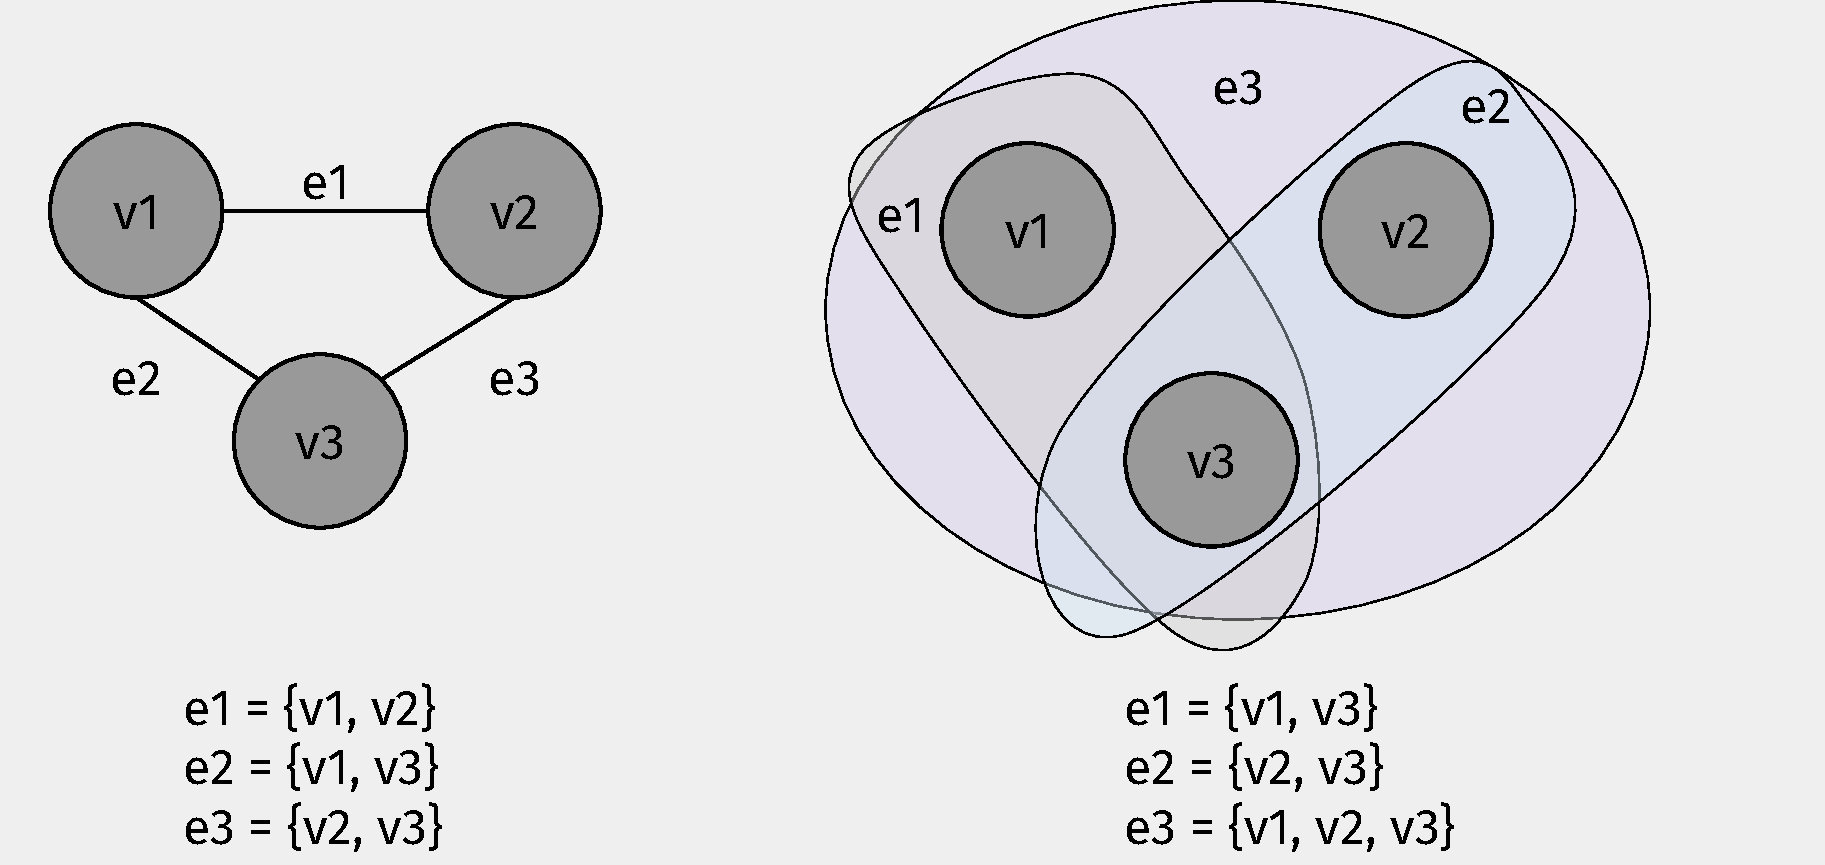
\includegraphics[width=0.7\linewidth]{images/Chapitre3/graph_vs_hgraph.pdf}
\caption{A graph (to the left) compared to a hypergraph (to the right). The edges of the hypergraph (hyperedges) may hold more than two nodes at once, relaxing the constraint of graphs' binary relations. A hypergraph can be seen as a set of $n$-ary sets: $E=\{\{v1,v3\},\{v2,v3\},\{v1,v2,v3\}\}$.}
\label{fig:graph_vs_hgraph}
\end{figure}


Building upon previous linguistic representations \cite{2007.Klapaftis.UOY,2011.Haishan.AHypergraphbased,2014.Tao.Qian.LexicalChainHypergraphWSI}, our model is indeed based on the use of a hypergraph.
% As stated before, hypergraphs have been employed in the literature to model complex systems. 
Their single most important difference with regular graphs, being able to relate more than two vertices at the same type, allows for a better characterization of interactions within a set of individual elements (in our case, words) \cite{heintz2014beyond}. Indeed, our hypergraph modelization initially integrates four types of relations between tokens: sentence co-occurrence, part-of-speech tags, words' constituents data and dependency relations in a single linguistic structure. These relationships were chosen because its is relatively easy to obtain them for high-resource languages. These features can be seen as building blocks for NLP models. Extracting deeper language features would implicate relying even more on general domain systems. In any case, our goal is to arrive to more complex annotations (e.g., named entities) from the selected features and relations. Indeed, as we discussed before, different types of contexts gives us different types of similarities. Recall that a shorter lexical window approximates us to a syntactical context. That is why we decided to keep a lexical context at sentence level, so that it may complement the distributional semantic information provided by the dependency functions context as well as the phrase-constituency syntactic context. In short, we  aim to cover three levels of possible semantic relatedness via  three levels (in terms of the size of the neighborhood of a target word) of distributional co-occurrences (see Figure \ref{}): with syntactic dependencies. a short range with dependency functions, a medium range with phrase constituency membership, and a longer range with sentence lexical co-occurrences. The intuition is that when solving NLP tasks, having direct access to these three semantic spaces will help to determine a more appropriate meaning's relation between words. 

 
\subsection{Construction}
In our case, the set of words in the corpus are the set of nodes  $V$, and the set of hyperedges  $E$ represent the relations between nodes according to different linguistic aspects.
%
We consider each word (i.e., each node) to exist in one of three types of hyperedges, two syntactic and one lexical co-occurrence contexts:
\begin{enumerate}
\item $\textsc{\textbf{NP}}$: noun phrase (NP)  constituents,
\item $\textsc{\textbf{DEP}}$: dependency relations: we consider all types of dependency functions between nouns and verbs,
\item  $\textsc{\textbf{SEN}}$: lexical context, in this case the window considered is the whole sentence
\end{enumerate} 

The part of speech information is stored implicitly with the constituent information. While these parameters are fixed in our implementation, they can easily be adapted to other configurations. For example, we may consider noun phrases and verb phrases as chunks, specific types of dependency functions, or different lexical window size.

To populate the hypergraph, given a token $v$, a noun phrase $p$, a sentence $s$, and a 
dependency function $dep(h, \cdot)$, with $h$ being the head of the relation, we consider the following rules:

\begin{itemize}
\item $v$ is incident (or belongs to a hyperedge $e_j$ of type $\textsc{\textbf{NP}}$ if  $v$ appears in the same noun phrase $p$.
\item The same condition is used with sentence hyperedges $\textsc{\textbf{SEN}}$: if  $v$ appears in a sentence $s$, it will be located in a hyperedge $e_j$ of type $\textsc{\textbf{SEN}}$. 
\item If $v$ participates in a dependency function $dep(h,v)$ as a dependent, it belongs to a hyperedge $e_j$ of type $\textsc{\textbf{DEP}}$.
\end{itemize}

Each hyperedge is labeled according to an identifier that allows the hypergraph to be populated while reading words from a corpus. For example, the hyperedges of the set $\textsc{\textbf{SEN}}=\{h_{S_1}, h_{S_2}, h_{S_3}\}$ are indeed hyperedges that represent sentences, identified by an index in this case. Hyperedges $h_{S_1}, h_{S_2}, h_{S_3}$ contain each a set of words. Additionally, the hypergraph can be represented as a $n \times m$ incidence $H$ matrix with entries $h(i,j) = N(v_i, e_j)$ where $N(v_i, e_j)$ is the number of times $v_i \in e_j$ occurs in the corpus. This frequency values can be later converted into other weighting schemes as seen in Chapter \ref{chap:backgnd}. Indeed, the incidence matrix allows us to pass from the hypergraph-based model of representation into the vector-space model.

\subsection{Running Example}
We illustrate the process of creating a sample hypergraph model with the following example phrase: \textit{The report contains copies of the minutes of these meetings}.  We tokenize the phrase, keeping all the words, and we lemmatize and parse it to obtain both constituency and dependency trees. For clarity, we  only show nouns as well as only the first three noun phrases, and the nominal subject (\textit{nsubj}) and direct object (\textit{dobj}) dependency relations.

\paragraph{Constituency Tree} The constituency tree of the example phrase is shown in Figure \ref{fig:tree}. The sentence, as well as each noun phrase (\textit{NP}) node is identified by a number, these numbers serve as an unique identifier of the phrase chunk within the whole sentence. We can observe that this phrase is composed by five noun phrases and one verb phrase. Meanwhile, some \textit{NP} are formed by other kind of phrases, depending on the grammar production rule used to build each one of them. Furthermore, as is usual in this kind of structures, there is a one to one relation between the number of tokens in the sentence  and the number of leaves in the tree. We see in total three hyperedges of this type: $NP_1, NP_2$ and $NP_3$, each corresponding to the noun phrases in the constituents tree.
 
\paragraph{Dependency Tree}
The dependencies of the example phrase are shown in Figure \ref{fig:tree_deps_report} as a tree structure. The relations can also be seen as tuples in Table \ref{tab:depends_report} In these relations' examples, the head is the first token to appear  followed by the dependent word. Two hyperedges are found: 
$nsubj_{contains}$ and $dobj_{contains}$.
 \begin{figure}
 \centering
 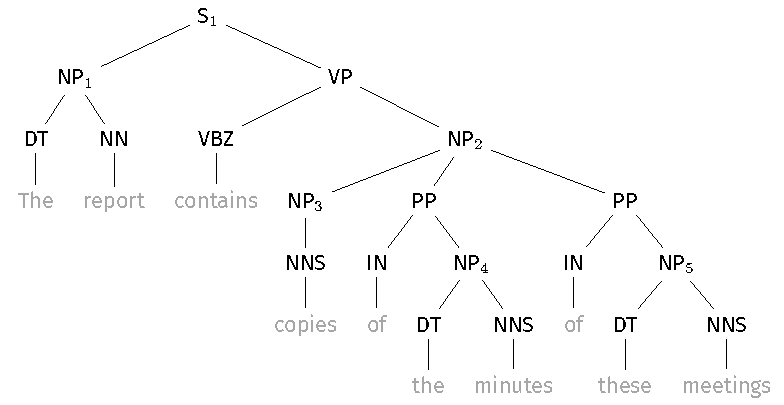
\includegraphics[width=0.7\linewidth]{images/Chapitre3/trees/tree_constits.pdf}
 \caption{Constituency-based tree of the phrase \textit{The report contains copies of the minutes of these meetings.}}
 \label{fig:tree_constits}
 \end{figure}
 
 %todo compare levels of semanticity in the three proposed models
 %
 
\begin{figure}[]
	\begin{minipage}{\textwidth}
		\begin{minipage}{.9\textwidth}
		\centering
		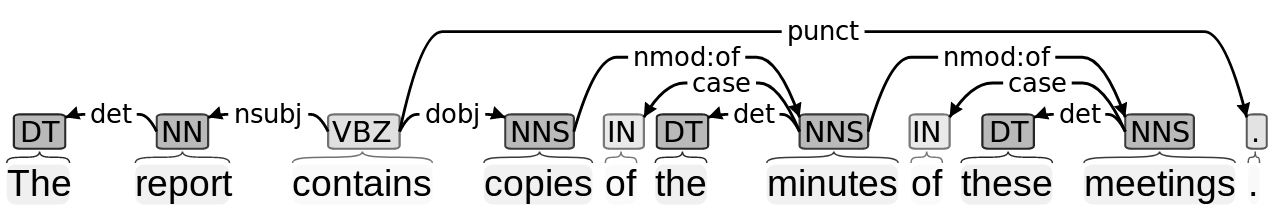
\includegraphics[width=0.9\linewidth]{images/Chapitre3/tree_deps_report.png}
		\captionof{figure}{Dependency-based tree of the example phrase.}
		\label{fig:tree_deps_report}
		\end{minipage} 
		\vspace{1cm}
		
		\begin{minipage}{.9\textwidth}
		\centering
		\begin{tabular}{@{}ll@{}}
%		 \toprule
		 \textbf{root}(root, contains)    & \textbf{det}(minutes, the)       \\
		 \textbf{det}(report, The)        & \textbf{nmod}(copies, minutes)   \\
		 \textbf{nsubj}(contains, report) & \textbf{case}(meetings, of)      \\
		 \textbf{dobj}(contains, copies)  & \textbf{det}(meetings, these)    \\
		 \textbf{case}(minutes, of)       & \textbf{nmod}(minutes, meetings)
		 \end{tabular}
		 \captionof{table}{Dependency relations of the example phrase.}
		 \label{tab:depends_report}
		\end{minipage} 
	\end{minipage}	
\end{figure}


 
\paragraph{Hyperdges Found}
From both syntactic parses and the phrase itself we build a hypergraph representation as stated before.  We show below the hyperedges sets found for each type,  ($\textsc{\textbf{NP}}$, $\textsc{\textbf{SEN}}$, and $\textsc{\textbf{DEP}}$), and their members. Each hyperedge  is labeled  with a unique identifier:

\begin{itemize}
\item $\textsc{\textbf{NP}}=\{NP_1, NP_2, NP_3\}$
	\begin{itemize}
		\item $NP_1=\{report\}$	
		\item $NP_2=\{copies,\,minutes,\,meetings\}$
		\item $NP_3=\{minutes\}$
	\end{itemize}
\item $\textsc{\textbf{SEN}}=\{S_1\}$
	\begin{itemize}
		\item $S_1=\{report,\,contains,\,copies,\,minutes,\,meetings\}$	
	\end{itemize}
\item $\textsc{\textbf{DEP}}=\{nsubj_{contains},\,dobj_{contains}\}$
	\begin{itemize}
		\item $nsubj_{contains}=\{report\}$	
		\item $dobj_{contains}=\{copies\}$	
	\end{itemize}

\end{itemize}

\paragraph{Incidence Matrix}We can represent these hyperedges as an incidence matrix, illustrated in Figure \ref{fig:incidence_report}.  
Looking at the table, we can   infer that the word \textit{copies} appears  in two hyperedges of type $\textsc{\textbf{NP}}$: first in \textit{NP$_2$}, which is built from a noun phrase  and two prepositional phrases (\textit{PP}). Secondly, we see that it is part of \textit{NP$_3$}, which  indicates a plural noun (\textit{NNS}).
Regarding the syntactic dependency hyperedges, the word \textit{copies} appear in the \textit{dobj} \textit{contains} column which indicates that \textit{copies} was the direct object of the verb \textit{contains}. Concerning the sentence hyperedges, we see that the token \textit{copies} appeared in the same sentence S$_1$ as the other four noun words.

\subsection{Discussion}
With the short example we show the intuitive way in which we identify three different kinds of relations: lexical co-occurrence (at sentence level), dependency co-occurrence, and noun phrase co-occurrence. Looking at the incidence matrix we see the three levels of semantic relatedness we aim to represent with the three different types of context: sentence, dependency, and noun phrase level. At the same time, there is a structure within the hypergraphs. Groups of words are found to be together either directly or by means of paths traced by other nodes. 

On the other hand, also looking a the matrix, we realize that it is sparse\footnote{Sparse for the  size of this example incidence matrix. Sparsity increases as more text is included in the hypergraph.}. Sparsity, as we saw previously, affects the performance of knowledge discovery techniques applied to NLP tasks. 

Just as the literature approaches covered before, we aim to solve semantic tasks by using the proposed linguistic resource and its relations. Yet, unlike those approaches we have three levels of semantic relatedness to dispose of and the $n$-ary relations from the hypergraph structure. 
% We can thus build systems that allow us to interpret a word from different perspectives according to said relations.


%In order to apply the proposed linguistic network to an input corpus we first need to parse it and thus obtain the required information from it to populate the hypergraph. In the following, we describe the method used to extract and store linguistic information from the English Wikipedia. %The procedure begins by extracting the text from an English Wikipedia dump and concludes by saving into disk the Wikipedia corpus in the format of our proposed language network (represented as a hypergraph incidence matrix with its complementary metadata information about the meaning of each vertex and hyperedge). 




\begin{figure}
\centering
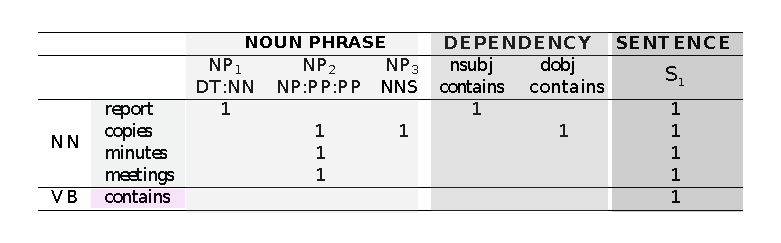
\includegraphics[width=\linewidth]{images/Chapitre3/incidence_mat.pdf}
\caption{Incidence matrix of the example phrase hypergraph modelization.}
\label{fig:incidence_report}
%todo change font to fira!
\end{figure}


\label{chap6:back}
 
We first describe below the fusion techniques we use in our methodology as well as relevant use cases where they have been employed. Then, we focus exclusively on fusion techniques applied to NLP tasks, which is the general domain of the two tasks (NER and WSI/WSD) we focus on.                                                                                                                 
\section{Multimodal Fusion Techniques}
Multimodal fusion is a set of popular techniques used in multimedia analysis tasks. T\textit{}hese methods integrate multiple media features, the affinities among these attributes or the decisions obtained from systems trained with said features, to obtain rich insights about the data being used and thus to solve a given analysis  task \cite{AtreyHEK10}. We note that these techniques come at the price of augmenting the complexity of a given system by increasing or reducing the sparsity of a given feature matrix.


In the multimodal fusion literature we can discern two main common types of techniques: early fusion and late fusion. 
\subsection{Early Fusion}
This technique is the most widely used fusion method. The principle is simple: we take both modal features and concatenate them into a single representation matrix. More formally, we consider two matrices  that represent different modality features each  over the same set of individuals. To perform early fusion we concatenate them column-wise, such that we form a new matrix having the same number of lines but increasing the number of columns to the sum of the number of columns of both matrices. The matrices may also be weighted as to control the influence of each modality.

The main advantage of early fusion is that a single unique model is fitted while leveraging the correlations among the concatenated features. The method is also easy to integrate into an analysis system. The main drawback is that we increase the representation space and may make it harder to fit models over it.
%

%   of shape $(n, m + p)$. Following the literature notation of [vulic], the early fusion representation matrix EF is defined as:
%\begin{equation}
%EF = \alpha \times X_1 || (1 - \alpha) \times X_2
%\end{equation}

%where $||$ represents the column-wise concatenation operation and ? is the parameter that determines the contribution of each modality. 
%
%Early fusion has been employed in several multimodal tasks. For example, [?]. 
\subsection{Late Fusion}
In contrast to early fusion, in late fusion the combination of multimodal features are generally performed at the decision level, i.e., using the output of independent models trained  each with an unique set of features \cite{ClinchantAC11}. In this setting,  decisions produced by each model are combined into a single final result set.
%
The methods used to combine preliminary decisions usually involve one of two types: rule-based (where modalities are combined according to domain-specific knowledge) or linear fusion (e.g., weighting and then adding or multiplying both matrices together). This type of fusion is very close to the so-called ensemble methods in the machine learning literature.
%
Late fusion combines both modalities in the same semantic space. In that sense,  we may also combine modalities via an affinity representation instead of final decision sets. In other words, we can combine two modality matrices by means of their respective similarities. A final representation is then usually obtained by adding the weighted similarity matrices.
%

The advantages of late fusion include the combination of features at the same level of representation (either the fusion of decisions or similarity matrices). Also, given that independent models are trained separately, we can chose which algorithm is more adequate for each type of
features.

%For example, in information retrieval (Ah-Pine et al., 2015), lexicon learning (Vulic et al., 2016), coreference resolution (Eisenstein and Davis, 2007); different types of representations (different modalities) can be combined in order to take advantage of the complementarity existing among them
\subsection{Cross-media Similarity Fusion}
%
A third type of fusion technique, cross-media similarity fusion (or simply cross fusion),   introduced in \cite{Ah-PineCC15,ClinchantAC11}, is defined and employed to propagate a single similarity matrix into a second similarity matrix. In their paper, the authors propagated information from textual media towards visual media. In our case, we transfer information among textual features. For example, to perform a cross fusion between lexical and syntactical features, we perform the following steps: 
\begin{enumerate}
\item Compute the corresponding similarity matrices for each type of feature.
\item Select only the $k$-nearest neighbor for each word within the lexical similarity matrix. These neighbors are to be used as lexical representatives to enrich the syntactical similarities.
\item Linearly combine both similarity matrices (lexical $k$-nearest lexical neighbors with the syntactical features) via a matrix product.
\end{enumerate}  

Cross fusion aims to bridge the semantic gap between two modalities by using the most similar neighbors as proxies to transfer valuable information  from one modality onto another one. Usually, the result of a cross fusion is combined with the previous techniques, early and late fusion. In this work we perform  experiment in that sense.

\subsection{Hybrid Fusion}
We may leverage the advantages of the previous two types of fusion techniques by combining them once more in a hybrid setting. As described in \cite{AtreyHEK10,yu2014informedia}, the main idea is to simultaneously combine features at the feature level, i.e., early fusion, and at the same semantic space or decision level. Nonetheless, they define a specific type of hybrid fusion. In this chapter, we adopt a looser definition of hybrid fusion. That is, we perform hybrid fusion by leveraging the combination of the fusion strategies described before.

In the following section we set to solve a natural language processing task using the model described above. Specifically, we address the word sense induction and disambiguation challenges. Both tasks are located on the computational semantics sub-domain of NLP. By making use of the network we want to test the effectiveness of using different types of linguistic features. 

